Para definir um valor para a concentração da superfície para implementação da solução clássica da Segunda Lei de Fick como descrito na Seção \autoref{sec:sol-numerica-2alei}, foi utilizado o artigo  \cite{christiansen2008nitrogen}, que possui o valor da ocupância de átomos de nitrogênio $y_N^{S}$ (mais especificamente a fração de interstícios octaédricos do reticulado cúbico de face centrada ocupada por nitrogênio) para o estado de equilíbrio, com $K_N=$2,49 $bar^{1/2}$ (valor para o qual os dados experimentais do artigo em questão mostravam-se mais próximos dos dados do modelo), para 445°C (718K). A variável $K_N=\dfrac{p_{NH_3}}{p_{H_2}^{3/2}}$ é o potencial de nitretação para uma mistura gasosa de NH$_3$/H$_2$.

A partir do valor de $y_N^{eq}$, para uma temperatura de 718K, é possível definir a concentração em $mols/m^3$ de nitrogênio utilizando a relação apresentada no apêndice A2 do artigo \cite{jespersen2016modelling}, dada pela equação\autoref{eq:oc-to-m3}.

\begin{equation} \label{eq:oc-to-m3}
	C = \dfrac{4}{N_A} \cdot y_N \cdot \dfrac{1}{V(y_N)}
\end{equation}

O fator 4 é o número de interstícios octaédricos de uma célula unitária CFC, $N_A$ é o número de Avogadro ($N_A = 6,0221409 \times 10^{23} (mol^{-1})$) e $V(y_N)$ é o volume da célula unitária (em $m^3$) para uma dada ocupância de nitrogênio.

A função $V(y_N)$ foi aproximada por uma função linear: 
\begin{gather*}
	V(y_N) = 2,8147 \times 10^{-29} \cdot y_N + 4,7134 \times 10^{-29}
\end{gather*}

Sendo assim, pode-se reescrever a equação \autoref{eq:oc-to-m3} como:

\begin{equation} \label{eq:oc-to-m3-full}
	C = \dfrac{4}{6,0221409 \times 10^{23}} \cdot \dfrac{y_N}{2,8147 \times 10^{-29} \cdot y_N + 4,7134 \times 10^{-29}}
\end{equation}

Dessa forma, para as condições especificadas acima, o valor de $y_N$ é 0,28 e a concentrção é 33.805 mol/m$^3$ (2,0358 $\times$ 10$^{28}$ m$^-3$).

\begin{table}[ht]
\centering
\setlength{\doublerulesep}{\arrayrulewidth}
{\def\arraystretch{2}\tabcolsep=10pt
\caption{Parâmetros para concentração na superfície constante}
\resizebox{\textwidth}{!}{
\begin{tabular}{c c c}
\hline\hline
Parâmetro & Descrição & Valor \\\hline

$C_{eq}$ & Concentração de equilíbrio entre gás e aço &  47.318,64 mol/m$^3$ (2,0358 $\times$ 10$^{28}$ m$^-3$)   \\
\hline\hline
\end{tabular}
\label{tab:parametros_csvar}
}
}
\end{table}

Os valores de $\Delta t$ e $\Delta x$ utilizados foram 0,01s e 0,1 $\mu m$. Para um tempo total de 22 horas e 20 $\mu m$ de profundidade, com temperatura igual a .



\begin{figure}[ht]
\centering
	\caption{Resultado simulação para concentração na superfície constante até 2 horas}
	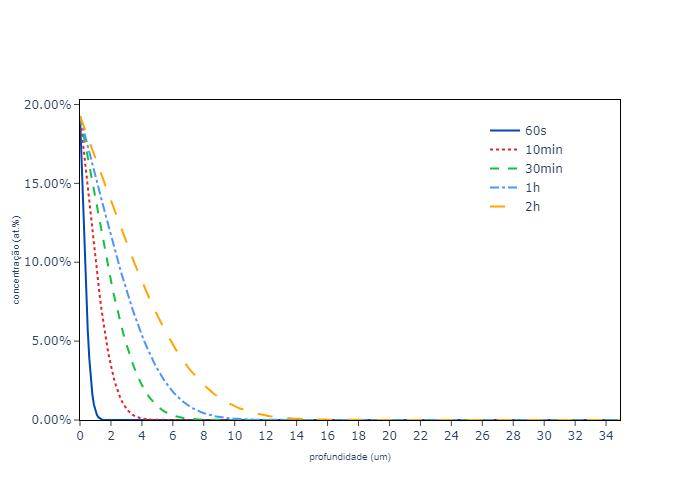
\includegraphics[width=1.0\textwidth]{plot_fickCte1}
	\label{fig:csvar-gas}
	\centering
	\fonte{Elaborado pela autora}
\end{figure}


\begin{figure}[ht]
\centering
	\caption{Resultado simulação para concentração na superfície constante até 22 horas}
	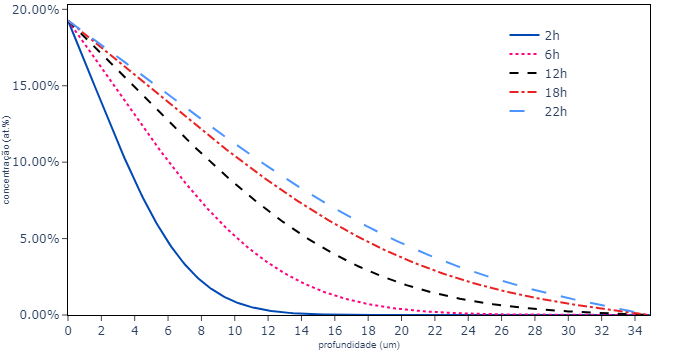
\includegraphics[width=1.0\textwidth]{plot_fickCte2}
	\label{fig:csvar-gas}
	\centering
	\fonte{Elaborado pela autora}
\end{figure}



\myworries{//escrever sobre os gráficos}